\documentclass[10pt,a4paper]{article} %#Establece el tipo de documento y sus especificaciones
%##Lista de paquetes que se podrán usar en el documento
\usepackage[left=2cm,right=2cm,top=2cm,bottom=2cm]{geometry}
\usepackage[dvipsnames]{xcolor}
\usepackage[fleqn]{mathtools}
\usepackage{booktabs}
\usepackage{amsmath}
\usepackage{latexsym}
\usepackage{graphicx}%##Paquete para llamar imagenes
\usepackage{nccmath}
\usepackage{multicol}
\usepackage{listings}
\usepackage{tasks}
\usepackage{color}
\usepackage{float}
\usepackage{lipsum}

\definecolor{colorIPN}{rgb}{0.5, 0.0,0.13}
\definecolor{colorESCOM}{rgb}{0.0, 0.5,1.0}
\graphicspath{ {imagenes/} }

\begin{document} %##Indica donde inicia el documento
	%#########################################################
	\begin{titlepage}
		\centering
		{ \huge \bfseries \color{colorIPN}{Instituto Politécnico Nacional} \par}
		{ \Large \bfseries  \color{colorESCOM}{Escuela Superior de Cómputo} \par }
		\vspace{1cm}%##Inserta una separación de tamaño exacto entre líneas
		{\huge\Large \color{colorIPN}{Web App Development}.\par}
		\vspace{1.5cm}
		{\huge\Large  \color{colorESCOM}{Ejercicio 1 : Instalar GIT}\par}
		\vspace{2cm}
		{\Large\itshape \color{colorIPN}{Profesor: M. en C. José Asunción Enríquez Zárate}\par} \hfill \break
		\vspace{2cm}
		{\Large\itshape \color{colorIPN}{Alumno: Mauro Sampayo Hernández}\par} \hfill \break
		{\Large\itshape \color{colorIPN}{mauro\_luigi@hotmail.com}\par} \hfill \break
		{\Large\itshape \color{colorIPN}{3CM18} \par}
		\vfill
		{\large \color{colorIPN}{3 de Septiembre del 2021}\par} 
		\vfill
	\end{titlepage}
	
	\renewcommand\lstlistingname{Quelltext} 
	
	
	\lstset{ 
		language=Java,
		basicstyle=\small\sffamily,%##Cambia la configuracipon del tipo de letra de forma permanente
		numbers=left,
		numberstyle=\tiny,
		frame=tb,
		tabsize=4,
		columns=fixed,
		showstringspaces=false,
		showtabs=false,
		keepspaces,
		commentstyle=\color{Violet},
		keywordstyle=\color{colorIPN} \bfseries,
		stringstyle=\color{colorESCOM}
	}
	
	\settasks{
		counter-format=(tsk[r]),
		label-width=4ex
	}
	\tableofcontents 
	\pagebreak
	
	\pagenumbering {arabic} %##Coloca el contador de páginas a 1 y comienza a numerar de acuerdo con el estilo especificado. En este casoi dicho estilo de numeracion es el arabigo
	
	\pagebreak
	
	%################################################
	\section{\color{colorIPN}{Introducción}}%##Crea secciones númeradas, en este caso esta es la seccion 1
	{\large La herramienta Git es el sistema de control de versiones moderno de mayor uso a nivel mundial y de  c{\' o}digo abierto. El uso de esta herramienta es indispensable debido a que los softwares cada d{\' i}a aumentan de complejidad, lo cual hace necesario el uso de mejores herramientas para llevar a cabo el control de cambios que se realicen a un software en espec{\' i}fico, as{\' i} como tambi{\' e}n el poder llevar a cabo el desarrollo de dicho software de manera coordinada entre varias personas. En este reporte se mostrar{\' a} el proceso de instalación y configuración de Git el cuál se encuentra especificado en la secci{\' o}n \ref{instal}.}
	
	%\subsection{ \color{colorESCOM}{Sub Sección 1}} %##Crea subsecciones numeradas
	%\lipsum[2-3] %##Añade tecto lorem ipsum
	
	\pagebreak
	
	%################################################
	\section{\color{colorIPN}{Conceptos}}
	{\large A continuaci{\' o}n se enlista una serie de conceptos, que son necesarios para poder entender m{\' a}s a detalle que es la herramienta Git, as{\' i} como tambi{\' e}n algunos de los componentes que la conforman y algunas de las configuraciones que se llevar{\' a}n a cabo en la secci{\' o}n \ref{instal}, donde se mostrar{\' a} el proceso de instalaci{\' o}n y configuraci{\' o}n de Git.}
	
	\subsection{ \color{colorESCOM}{Git Bash}}
	{\large Es una aplicaci{\' o}n para entornos de Microsoft Windows que ofrece una capa de emulaci{\' o}n para una experiencia de l{\' i}neas de comandos de Git.}
	
	\subsection{ \color{colorESCOM}{Shell}}
	{\large Shell es una aplicaci{\' o}n de terminal que se utiliza como interfaz con un Sistema Operativo mediante comandos escritos.}
	
	\subsection{ \color{colorESCOM}{Repositorio}}
	{\large Es un sitio centralizado donde se almacena y mantiene informaci{\' o}n digital, habitualmente bases de datos o archivos inform{\' a}ticos.}
	
	\subsection{ \color{colorESCOM}{Entorno de Desarrollo (IDE))}}
	{\large Es aquel entorno digital empleado para desarrollar cualquier tipo de software cuyo objetivo es agilizar todo el proceso de dise{\~{n}}o de software, ofreciendo un servicio integral al programador.}
	
	\pagebreak
	
	%################################################
	\section{\color{colorIPN}{Desarrollo}}\label{instal}
	{\large Para el desarrollo de este ejercicio se mostrar{\' a} el proceso para llevar a cabo la correcta instalaci{\' o}n y configuraci{\' o}n de Git dentro de un Sistema Operativo Windows:}
	
	\begin{enumerate}
		{\large
			\item Se inicia ingresando a la liga \underline{https://git-scm.com/} en la cual se descarga el instalador de la versi{\' o}n m{\' a}s actual de Git.
			\begin{figure}[H]
				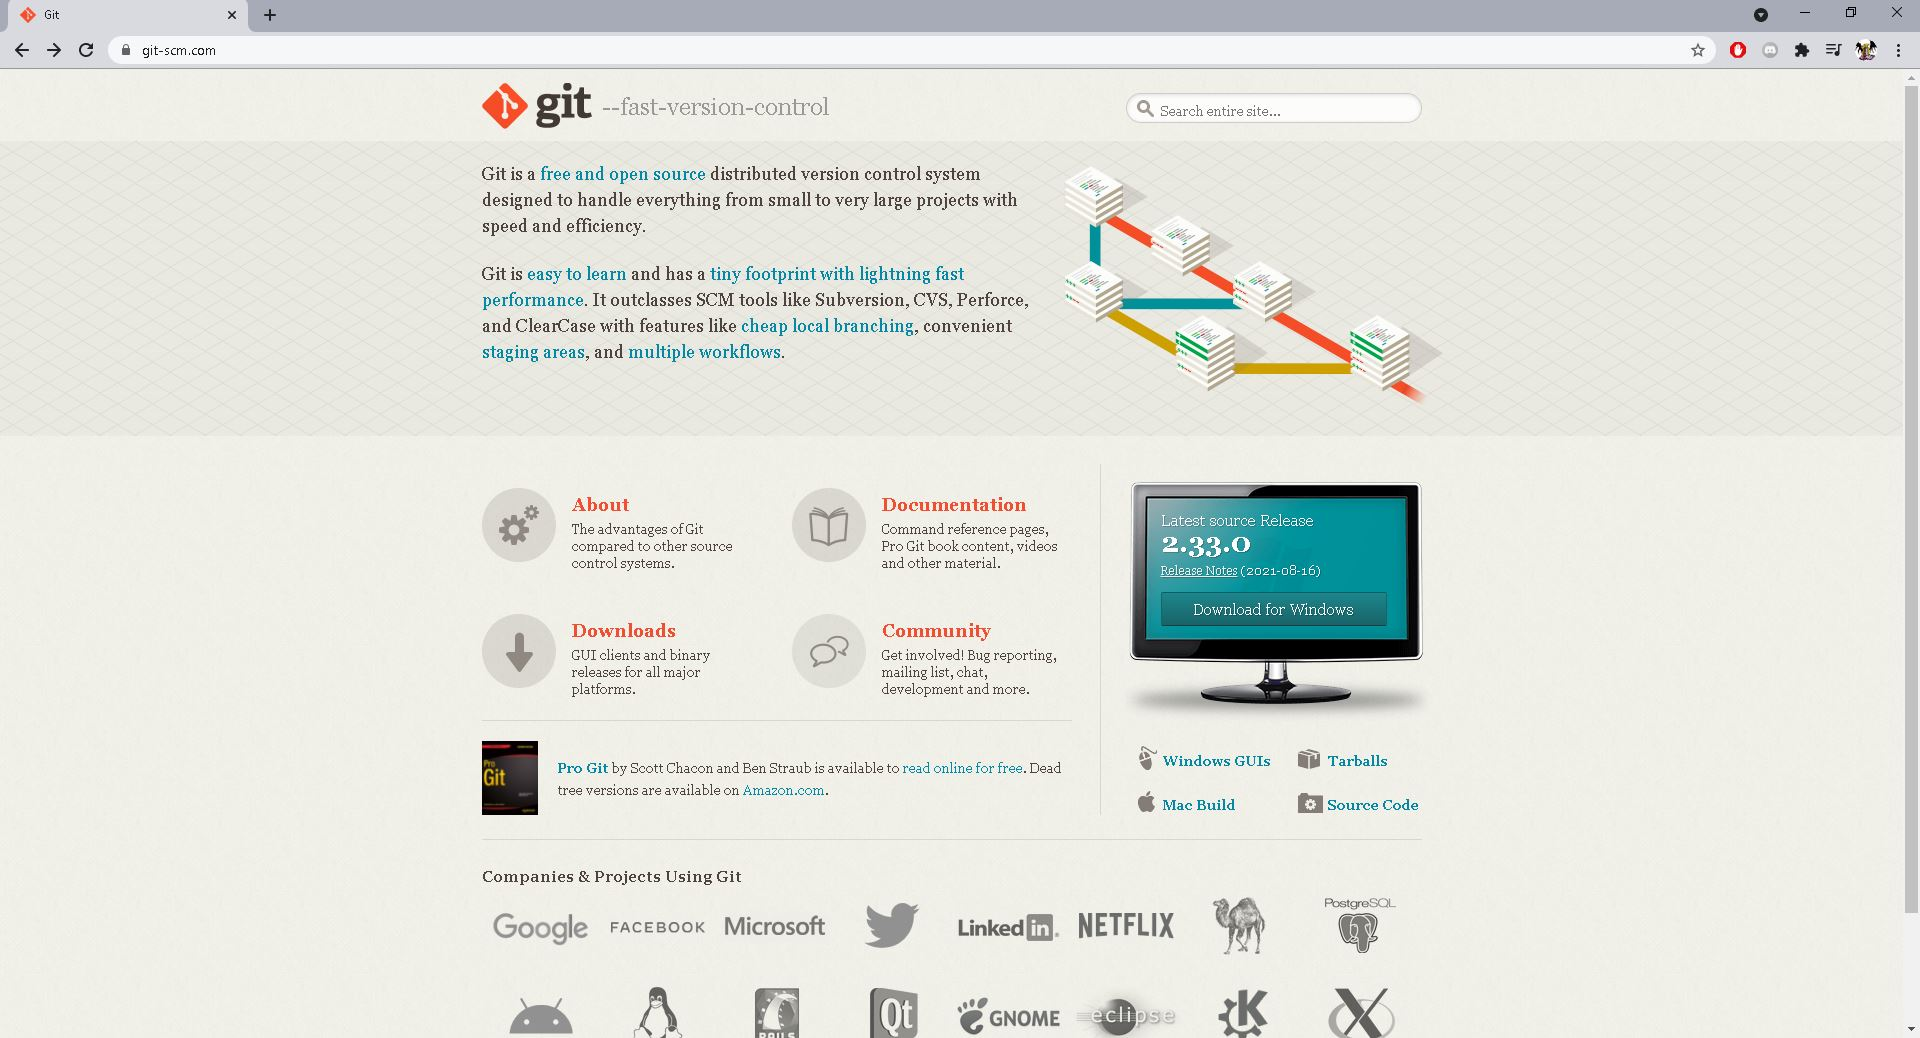
\includegraphics[width=0.8\textwidth]{1.jpg}
				\centering
				\label{img:paso1}
			\end{figure}
			\item Se nos redirige a una p{\' a}gina donde se iniciar{\' a} la descarga del instalador de Git.
			\begin{figure}[H]
				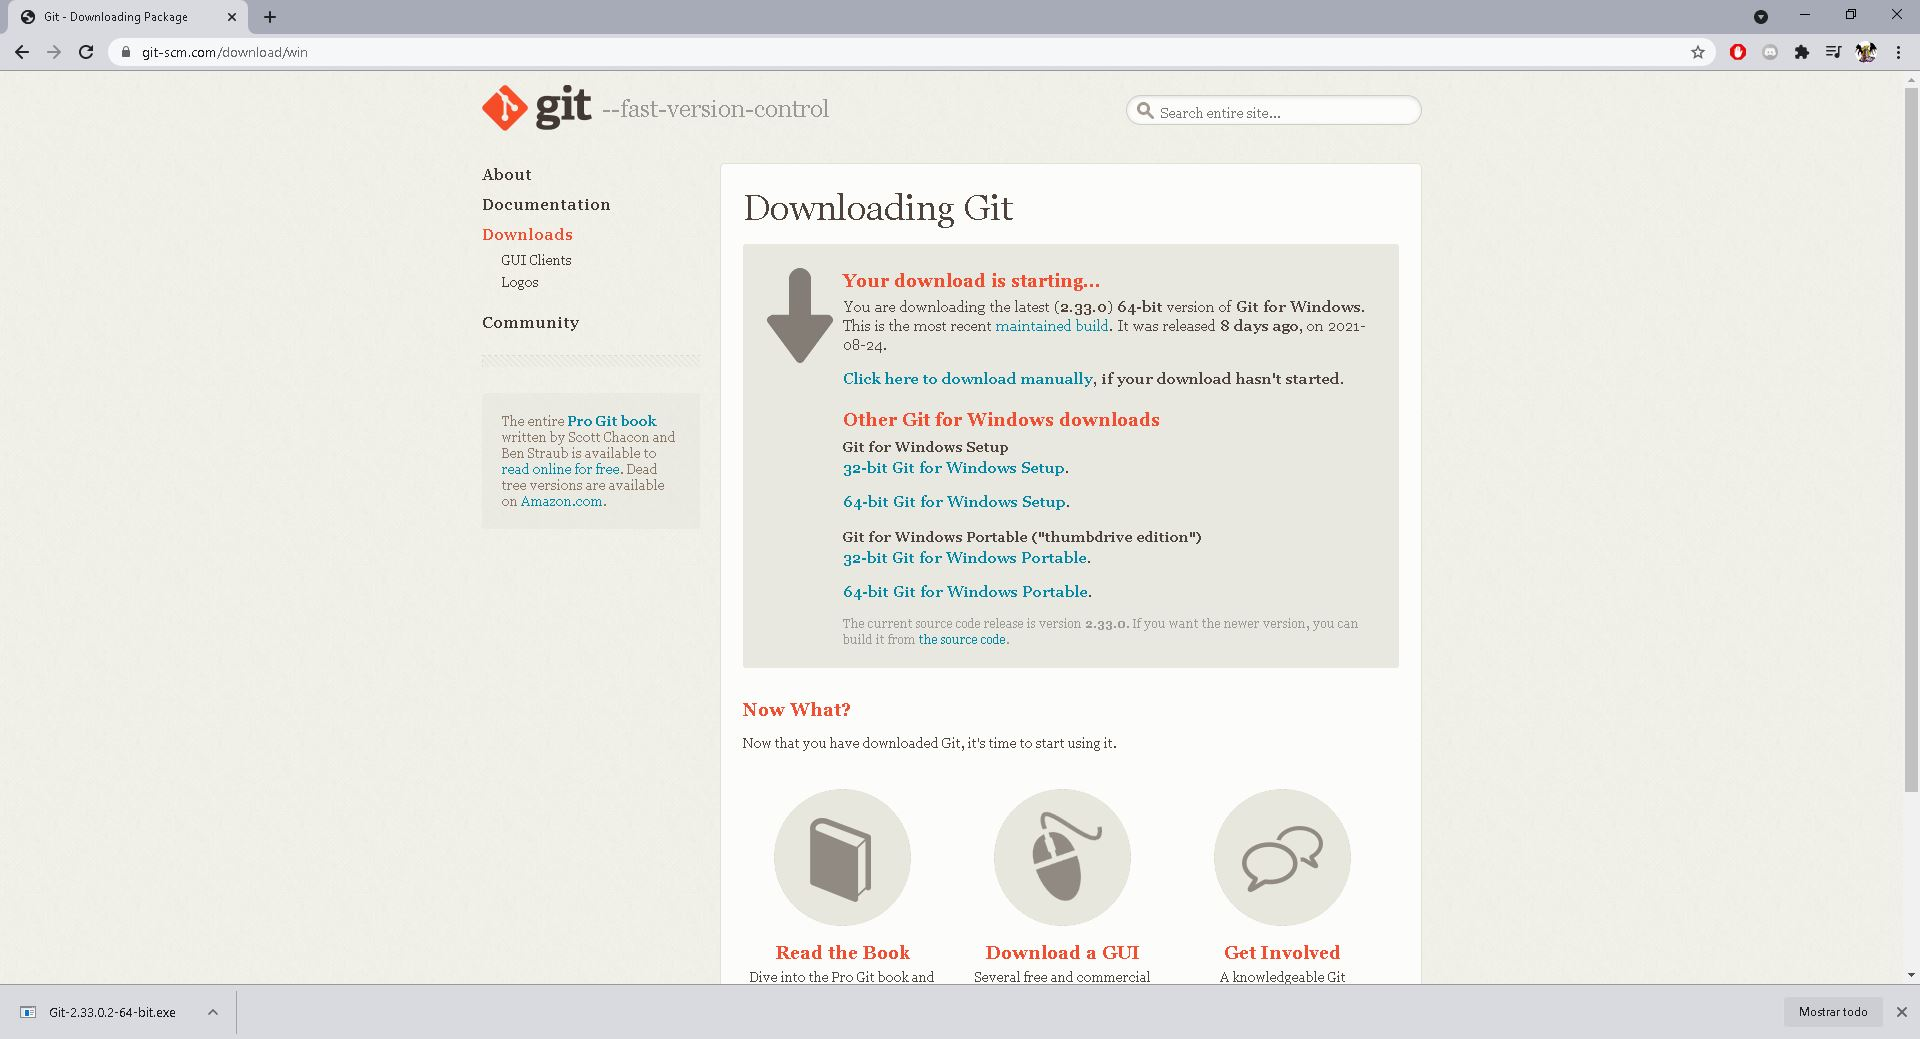
\includegraphics[width=0.8\textwidth]{2.jpg}
				\centering
				\label{img:paso2}
			\end{figure}
			
			\pagebreak
			\item Una vez haya finalizado la descarga del instalador, lo ejecutamos y se abrir{\' a} una advertencia de seguridad en la cual se debe seleccionar la opción ``Ejecutar".
			\begin{figure}[H]
				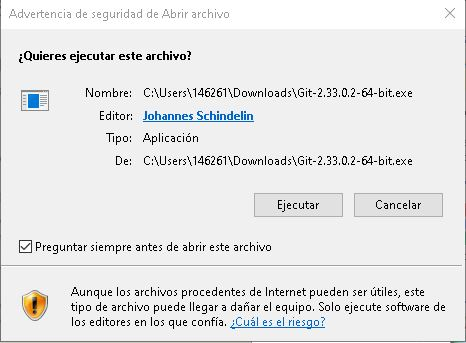
\includegraphics[width=0.6\textwidth]{3.jpg}
				\centering
				\label{img:paso3}
			\end{figure}
			\item Posteriormente debemos permitir que la aplicaci{\' o}n realice cambios en el dispositivo, para que as{\' i} pueda iniciarse la ejecuci{\' o} del instalador. La primera ventana nos mostrar{\' a} los t{\' e}rminos y condiciones a aceptar del programa. Se debe seleccionar la opción ``Next".
			\begin{figure}[H]
				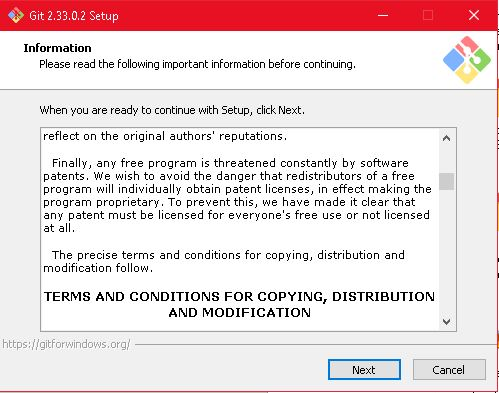
\includegraphics[width=0.6\textwidth]{4.jpg}
				\centering
				\label{img:paso4}
			\end{figure}
			
			\pagebreak
			\item La siguiente ventana nos da la opci{\' o}n de elegir localizaci{\' o}n de la carpeta en la que se quiera instalar Git, para este caso la localizaci{\' o}n de dicha carpeta se dejar{\' a} como viene por defecto. Posteriormente se debe seleccionar la opci{\' o}n ``Next".
			\begin{figure}[H]
				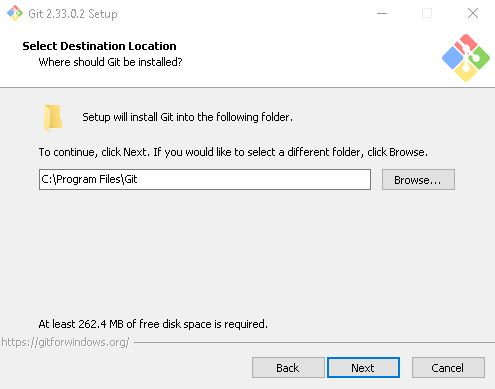
\includegraphics[width=0.6\textwidth]{5.jpg}
				\centering
				\label{img:paso5}
			\end{figure}
			\item La posterior ventana nos da la opci{\' o}n de seleccionar de una serie de componentes que pueden ser instalados para Git. En este caso se dejar{\' a} la configuraci{\' o}n que viene predeterminada y se seleccionara la opci{\' o}n ``Next".
			\begin{figure}[H]
				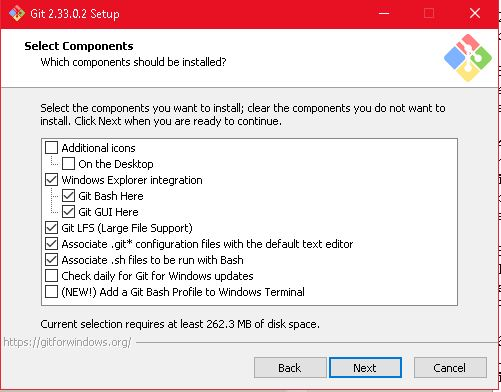
\includegraphics[width=0.6\textwidth]{6.jpg}
				\centering
				\label{img:paso6}
			\end{figure}
			
			\pagebreak
			\item La ventana que se presenta a continuaci{\' o}n nos da la opci{\' o}n de elegir la carpeta en donde se guardar{\' a} el acceso directo al programa. En este caso se dejar{\' a} el que ya viene establecido por defecto para despu{\' e}s seleccionar{\' a} ``Next".
			\begin{figure}[H]
				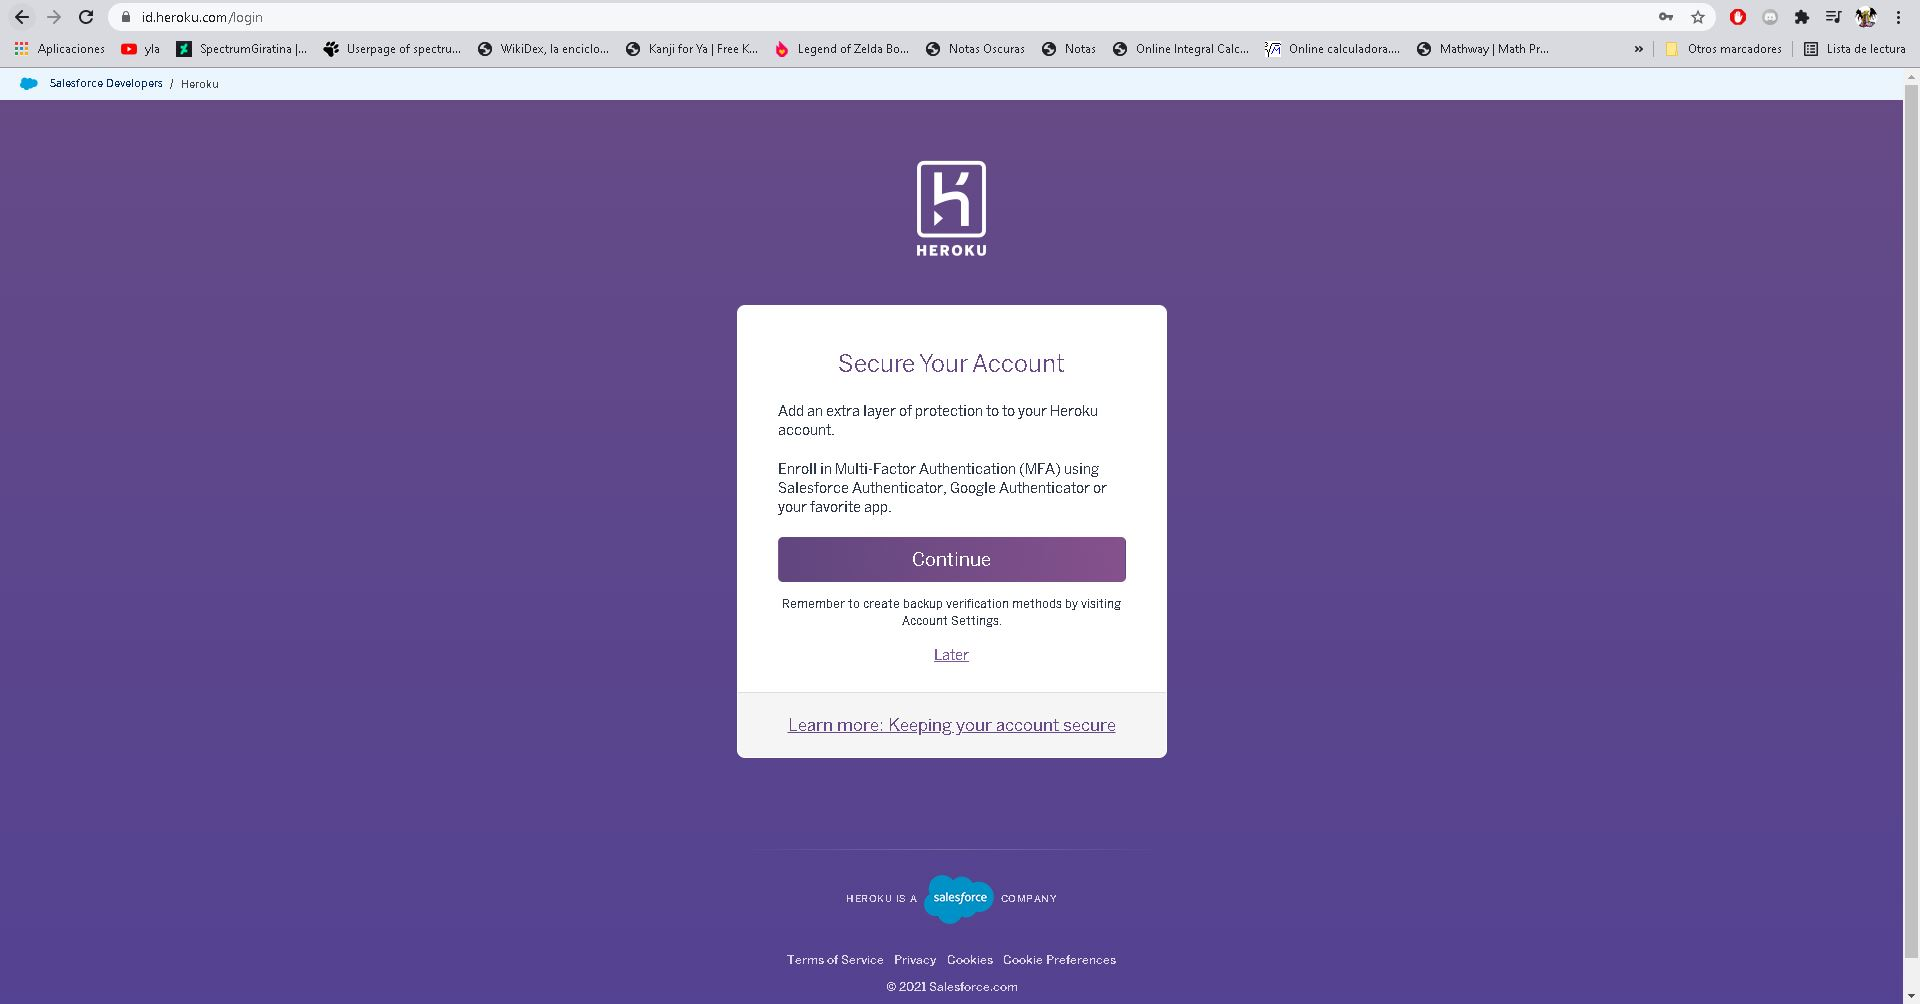
\includegraphics[width=0.6\textwidth]{7.jpg}
				\centering
				\label{img:paso7}
			\end{figure}
			\item Posteriormente se nos pide que seleccionemos el editor por defecto en el que se har{\' a} uso de Git, de una lista desplegable y la cu{\' a}l queda a preferencia del usuario. Para este caso se seleccionar{\' a} la opci{\' o}n de usar Sublime Text como editor por defecto. Se selecciona la opción de ``Next".
			\begin{figure}[H]
				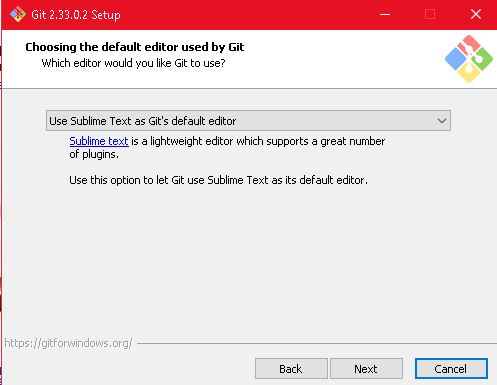
\includegraphics[width=0.6\textwidth]{8.jpg}
				\centering
				\label{img:paso8}
			\end{figure}
			
			\pagebreak
			\item En el siguiente paso se le debe de asignar un nombre a la rama principal, la cual se crear{\' a} cada vez que un proyecto en Git sea inicializado. Es posible ya sea asignar nosotros el nombre de dicha rama o dejar que Git decida por nosotros, en este caso se dejar{\' a} que Git decida. Se selecciona la opci{\' o}n de ``Next".
			\begin{figure}[H]
				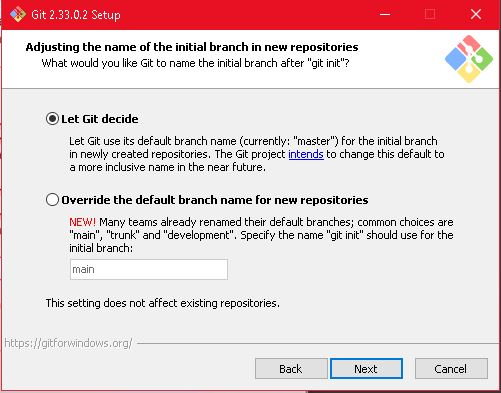
\includegraphics[width=0.6\textwidth]{9.jpg}
				\centering
				\label{img:paso9}
			\end{figure}
			\item La ventana siguiente nos deja elegir que entornos de desarrollo podr{\' a}n hacer uso de Git. Las opciones que se nos presentan en esta pantalla son:
			\begin{itemize}
				{
					\item Hacer uso {\' u}nicamente del bash de Git
					\item Utilizar Git desde una l{\' i}nea de comandos y/o desde programas de terceros
					\item Utilizar Git y las herramientas opcionales de Unix en la consola de comandos
				}
			\end{itemize}
			Para este caso se seleccionar{\' a} la segunda opci{\' o}n al ser la que m{\' a}s se adec{\' u}a a la materia. Se selecciona la opci{\' o}n de "``Next".
			\begin{figure}[H]
				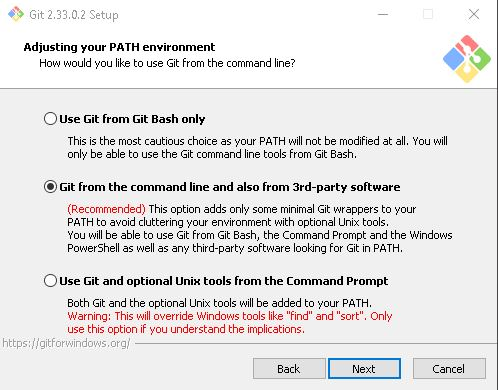
\includegraphics[width=0.6\textwidth]{10.jpg}
				\centering
				\label{img:paso10}
			\end{figure}
			
			\pagebreak
			\item En la siguiente pantalla se nos da a elegir si se quiere hacer uso de la Shell de OpenSSH que viene por defecto en Git, o si se desea usar alguna Shell externa, en este caso se seleccionar{\' a} la primera opci{\' o}n. Se selecciona la opci{\' o}n de ``Next".
			\begin{figure}[H]
				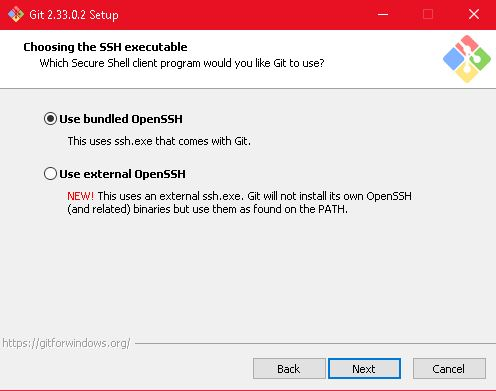
\includegraphics[width=0.6\textwidth]{11.jpg}
				\centering
				\label{img:paso11}
			\end{figure}
			\item En la posterior pantalla se nos pregunta sobre que librer{\' i}a se desea utilizar para realizar la comunicaci{\' o}n desde nuestra máquina remota con repositorios externos. En este caso se seleccionar{\' a} la opci{\' o}n de usar la librería OpenSSL. Se selecciona la opci{\' o}n de ``Next".
			\begin{figure}[H]
				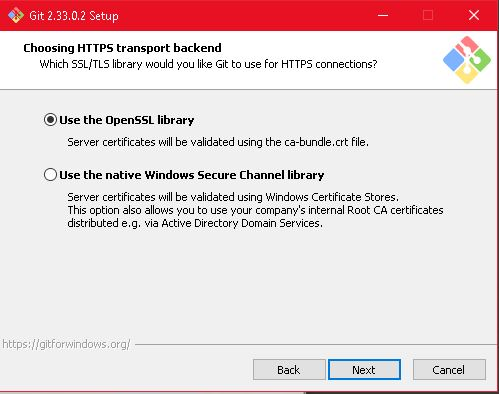
\includegraphics[width=0.6\textwidth]{12.jpg}
				\centering
				\label{img:paso12}
			\end{figure}
			
			\pagebreak
			\item Posteriormente se nos da a elegir la manera en la que se quiera manejar los saltos de l{\' i}nea, ya que estos se manejan de manera distinta dependiendo del Sistema Operativo que este en uso. La opci{\' o}n más recomendable es dejar que Git haga una conversi{\' o}n desde cada Sistema Operativo a Unix (primera opci{\' o}n). Se selecciona la opci{\' o}n de ``Next".
			\begin{figure}[H]
				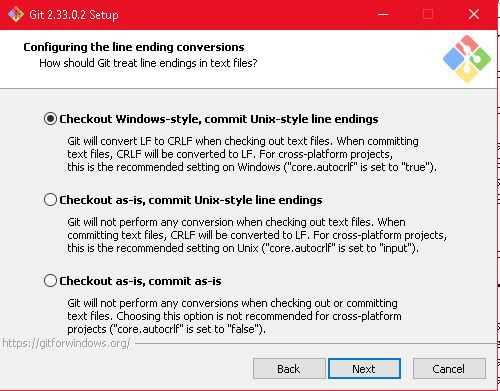
\includegraphics[width=0.6\textwidth]{13.jpg}
				\centering
				\label{img:paso13}
			\end{figure}
			\item Ahora se debe realizar la configuraci{\' o}n de la terminal que se desee utilizar en Git Bash. Se nos da la opci{\' o}n de usar la terminal bash propia de Git o  de usar la consola de Windows por defecto; en este caso se elige la opci{\' o}n m{\' a}s conveniente,m la cual es la primera y se selecciona la opci{\' o}n de ``Next".
			\begin{figure}[H]
				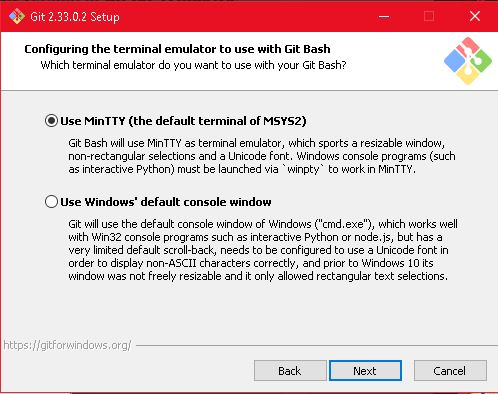
\includegraphics[width=0.6\textwidth]{14.jpg}
				\centering
				\label{img:paso14}
			\end{figure}
			
			\pagebreak
			\item En el posterior paso se nos pregunta acerca de c{\' o}mo se quiere que sea el comportamiento por defecto cuando se haga un "Git Pull" (comando que nos permite traer archivos o cambios que se tengan en un repositorio remoto). Lo m{\' a}s recomendable es dejar esta opci{\' o}n por default (fast-forward or merge) la cual se seleccionar{\' a} para este ejercicio. Se selecciona la opci{\' o}n de ``Next".
			\begin{figure}[H]
				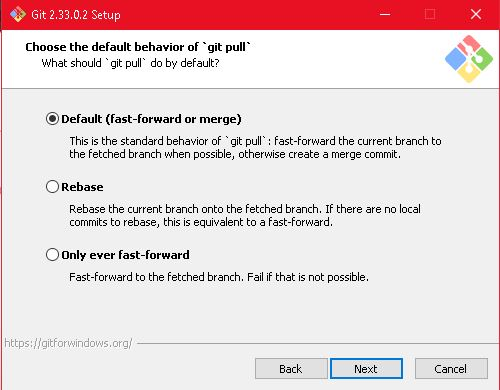
\includegraphics[width=0.6\textwidth]{15.jpg}
				\centering
				\label{img:paso15}
			\end{figure}
			\item Despu{\' e}s se nos pregunta acerca del manejador de credenciales relacionados a la cuenta de GitHub del usuario. Se dejar{\' a} seleccionada la opci{\' o}n por defecto y se seleccionar{\' a} la opci{\' o}n de ``Next".
			\begin{figure}[H]
				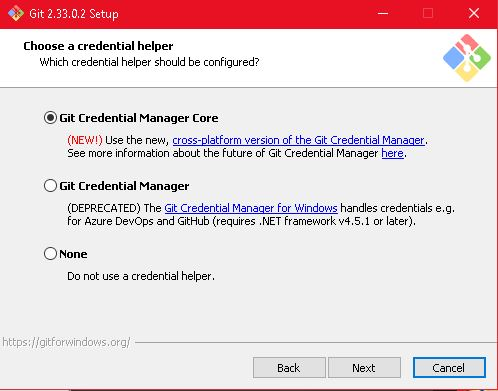
\includegraphics[width=0.6\textwidth]{16.jpg}
				\centering
				\label{img:paso16}
			\end{figure}
			
			\pagebreak
			\item Posteriormente se nos pregunta acerca de la configuraci{\' o}n de algunas opciones extra, dichas opciones son:
			\begin{itemize}
				{
					\item Habilitar el cach{\' e} del sistema
					\item Habilitar los links simb{\' o}licos
				}
			\end{itemize}
			Se puede seleccionar cuales de estas configuraciones se desea mantener habilitada o deshabilitada. Debido a que no se har{\' a} uso de los links simb{\' o}licos solo se dejar{\' o} habilitado el cach{\' e} del sistema. Seleccionamos la opci{\' o}n ``Next".
			\begin{figure}[H]
				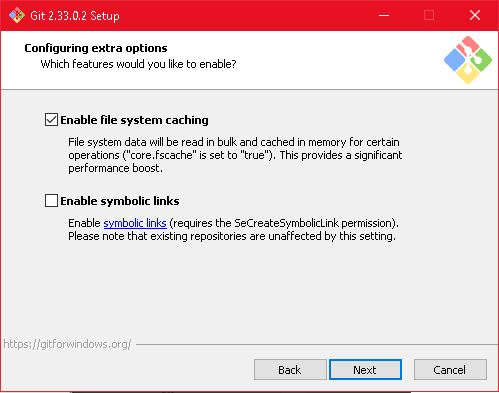
\includegraphics[width=0.6\textwidth]{17.jpg}
				\centering
				\label{img:paso17}
			\end{figure}
			\item Finalmente se nos pregunta acerca de la configuraci{\' o}n de algunas opciones extra en fase experimental. Para este caso no se habilitar{\' a} ninguna por lo que se proceder{\' o} a seleccionar la opci{\' o}n ``Install".
			\begin{figure}[H]
				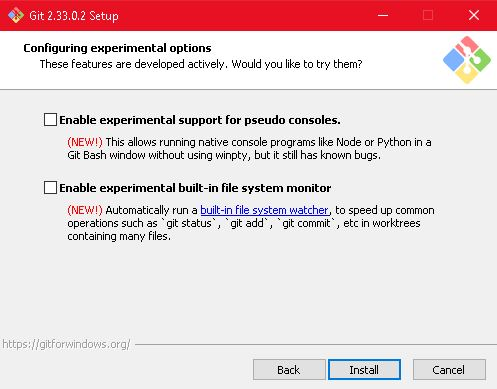
\includegraphics[width=0.6\textwidth]{18.jpg}
				\centering
				\label{img:paso18}
			\end{figure}
			
			\pagebreak
			\item Se inicializar{\' a} y concretar{\' a} el proceso de instalaci{\' o}n.
			\begin{figure}[H]
				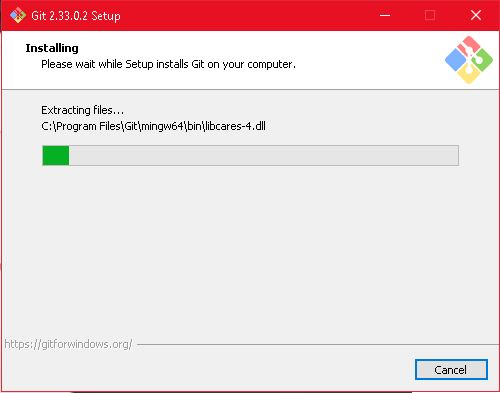
\includegraphics[width=0.6\textwidth]{19.jpg}
				\centering
				\label{img:paso19_1}
				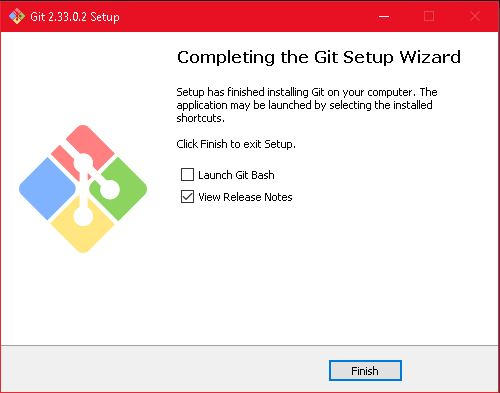
\includegraphics[width=0.6\textwidth]{19_2.jpg}
				\centering
				\label{img:paso19_2}
			\end{figure}
		}
	\end{enumerate}
	
	\pagebreak
	
	%################################################
	\section{\color{colorIPN}{Resultados}}
	{\large Al finalizar el proceso de instalaci{\' o}n y configuraci{\' o}n de Git podremos ejecutar el terminal Git Bash donde ser{\' a} posible realizar la ejecuci{\' o}n de comandos Unix.}
	
	\begin{figure}[H]
		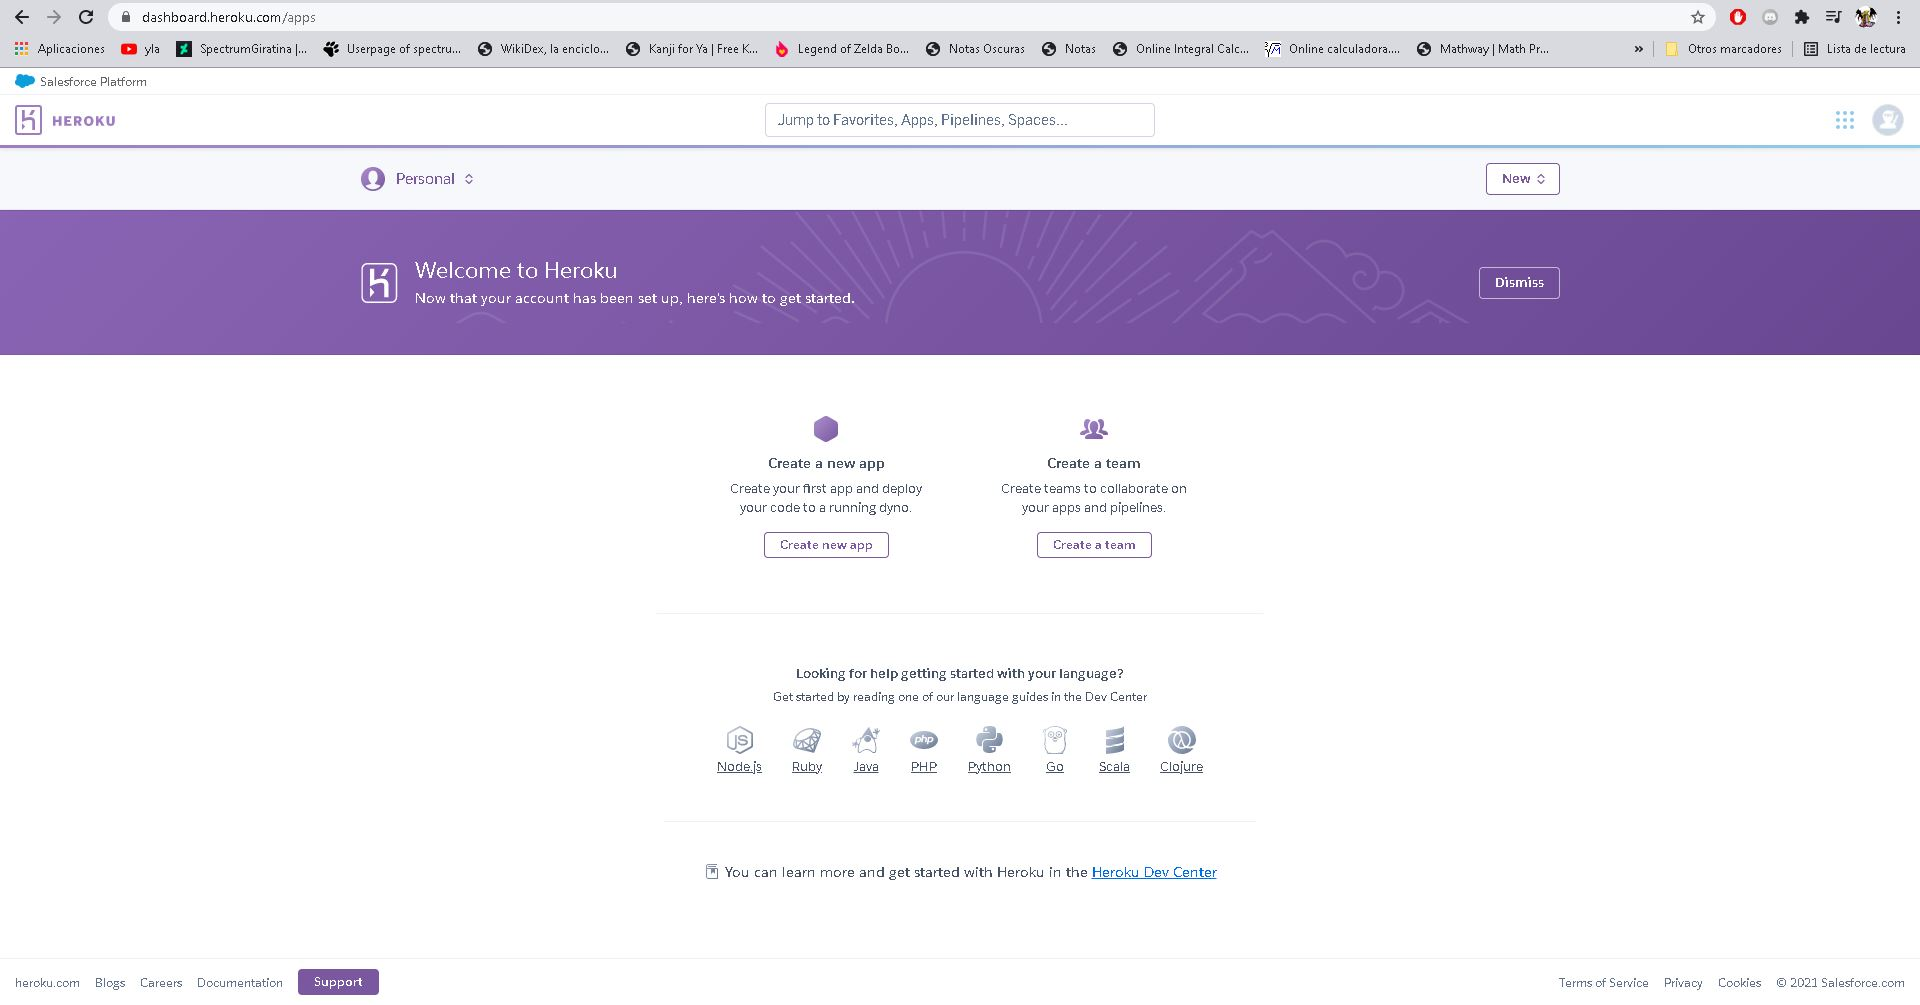
\includegraphics[width=0.8\textwidth]{resultado.jpg}
		\centering
		\caption{Terminal Git Bash}
		\label{img:resultado}
	\end{figure}  \hfill
	
	\pagebreak
	
	
	%################################################
	\section{\color{colorIPN}{Conclusión}}
	{\large Git resulta ser una herramienta bastante {\' u}til ya que nos permite alojar archivos inform{\' a}ticos en un repositorio, desde el cu{\' a}l se puyeden realizar modificaciones, llevando un control en dichos cambios que se realicen, as{\' i} como tambi{\' e}n guardar copias de versiones anteriores del software en caso de que se lleguen a necesitar. Dichos atributos resultan bastante {\' u}tiles al momento de llevar a cabo el desarrollo de softwares, al permitir una coordinación mucho más sencilla y un manejo más fácil del mismo durante su desarrollo.}
	
	\color{colorIPN}{
		\begin{flushright}
			\textit{
				Mauro Sampayo Hern{\' a}ndez
			}
		\end{flushright} \hfill \break
	}
	
	\pagebreak
	
	%################################################
	
	\section{\color{colorIPN}{Referencias Bibliográficas}}
	\color{colorESCOM}{
		\begin{thebibliography}{10}
			\bibitem {gitbash}
			\newblock {\em Git Bash}
			\newblock \textbf {Atlassian.}
			\newblock [accesed 2021 Sep 02]
			\newblock {\em https://www.atlassian.com/es/git/tutorials/git-bash}
			
			\bibitem {repositorio}
			\textbf {(2021)}
			\newblock {\em ¿Qué es un repositorio?}
			\newblock\textbf {ICTEA.}
			\newblock [accesed 2021 Sep 02]
			\newblock {\em https://www.ictea.com/cs/index.php?rp=/knowledgebase/3481/iQue-es-un-repositorio.html}
			
			\bibitem{Git}
			\newblock [accesed 2021 Sep 02]
			\newblock {\em https://git-scm.com/}
		\end{thebibliography}
	}
	
\end{document} %##Indica donde termina el documento
